\documentclass [hw,addpoints,noanswers]{exam}

\usepackage[hw]{physics9}


\title{Asynchronous assignment: Momentum data analysis}
\author{\mobeardInstructorShort}
\date{\printdate{4/27/2021}}
\duedate{\printdate{4/29/2021}}

\sisetup{separate-uncertainty=true,per-mode=symbol}


\begin{document}
\maketitle

\begin{abstract}
In physics and in future classes (notably chemistry and biology, but also any future science or math class and even many social science classes), you will need to be able to take data that has been gathered, generate graphs of the data, and use these graphs to answer questions. For this asynchronous assignment, you will gain practice using two different programs to visualize time series data for an inelastic collision, and to prepare a bar plot of the change in momentum. You should do your best to use the software; please do not try to draw the figures by hand. 
\end{abstract}

\begin{questions}
\question \textbf{Vernier Graphical Analysis (Results figure \#2).} 
\begin{parts}
\part Install the Vernier Graphical Analyiss app. On a Mac the link is here: \url{https://www.vernier.com/product/graphical-analysis-4/}. On iPad you can obtain the app through the App Store. 
\part Download the file \lstinline{inelastic.gambl} and open it in Vernier Graphical Analysis. 
\part The data should plot automatically, but you may need to adjust the axis labels or the plot ranges. Adjust the axis labels and plot ranges to something reasonable for this data.
\part Export your plot as a portable network graphic file named as follows: \lstinline{inelastic-lastname.png}, e.g. \lstinline{inelastic-smith.png}. You will submit this through Google Classroom.  Your plot may look like \fref{fig:elastic}. 
\part Write a descriptive caption for your plot.
\end{parts}

\question \textbf{Google Sheets (Results figure \#3).} Sometimes the data are collected through some other means where the Graphical Analysis app is not the most convenient way to plot it. One commonly used type of analysis program is a spreadsheet, such as Google Sheets, Microsoft Excel, Apple Numbers, etc. 
\begin{parts}
\part Download the file \lstinline{momentum-data-1-3.csv}. This file was collected from 72 runs by a mostly-friendly scientist; most data are correct but some may be wonky. If you decide some datapoints are wonky, you may toss them but you must explain why and how you decided what to toss. 
\part Construct columns to compute $p_0$, $p_f$, and $\Delta p$ according to the following:
\begin{align}
p_0 &= m_1 v_1 + m_2 v_2 \\
p_f &= m_1 v_{1,f} + m_2 v_{2,f} \\
\Delta p &= p_f - p_0
\end{align}

You will need to use cell references, e.g. the contents of cell \lstinline{G2} might be \lstinline{A2*C2+B2*D2} to give $p_0$, while the contents of cell \lstinline{H2} might be \lstinline{A2*E2+B2*F2} to give $p_f$. To obtain $\Delta p$ you might set \lstinline{I2} to \lstinline{H2-G2}. You can then copy the cells down the entire range. 

\part Determine the mean (\lstinline{AVERAGE()}) and standard deviation (\lstinline{STDEV()}) of $\Delta p$ and make a bar chart of these. Export your bar chart as \lstinline{momentum-change-lastname.png}, e.g. \lstinline{momentum-change-simpson.png}. You will submit these through Google Classroom.  Your plot may look like \fref{fig:momentum-change}
\part Write a descriptive caption for your plot.
\part Adventurous students may try using a $t$-test (\lstinline{TTEST()}) on the data. Google it!
\end{parts}
\end{questions}

\textbf{These are due on Thursday, \printdate{4/29/2021} to be submitted via Google Classroom; the results will then be included in a writeup of the momentum findings, which you will have two weeks to complete (major lab grade).}

\begin{figure}[p]
\begin{center}
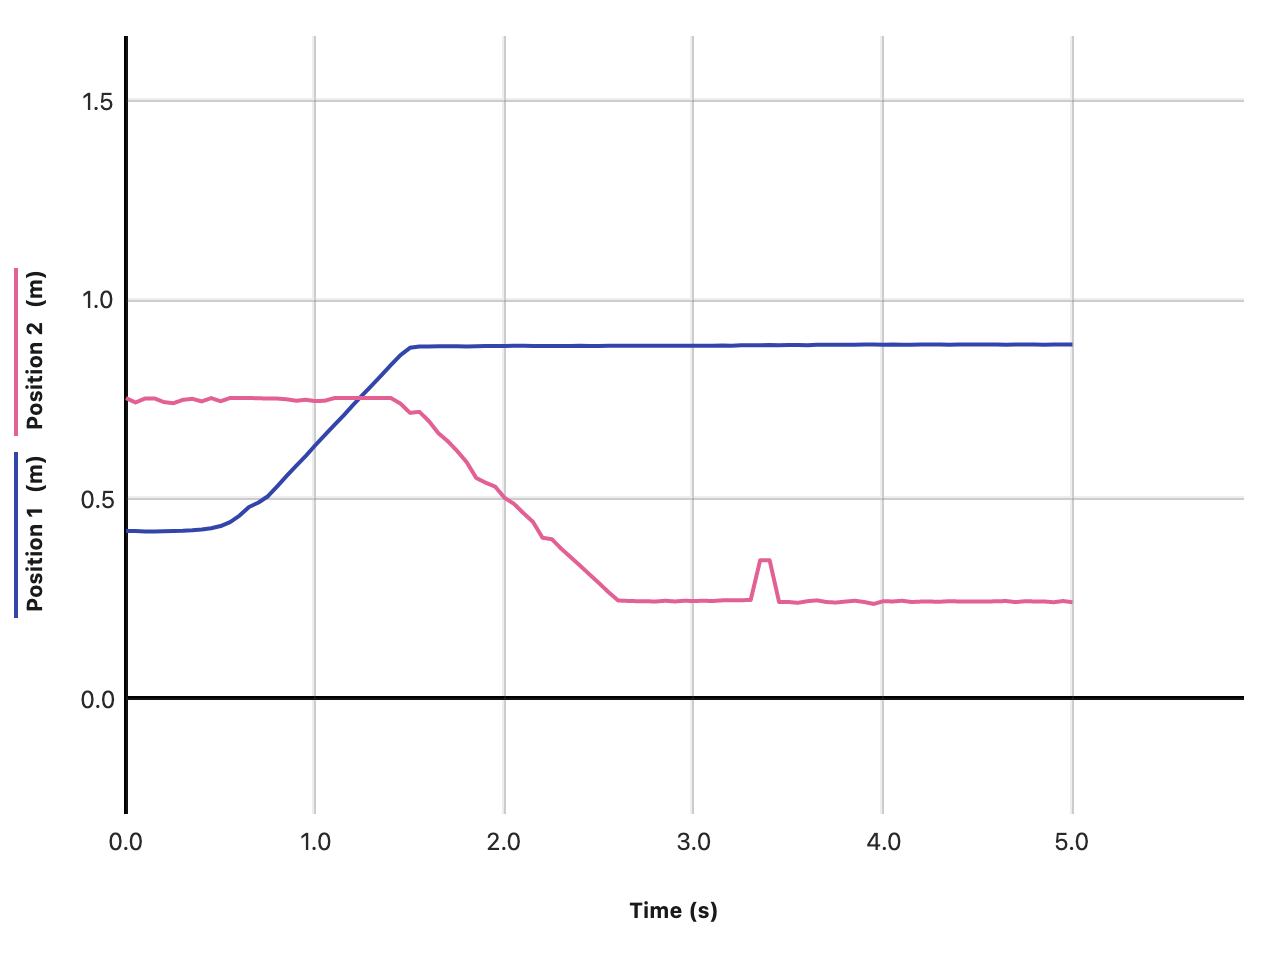
\includegraphics[width=4in]{elastic.png}
\end{center}
\caption{Example collision time series data for position. This particular plot is for an elastic collision, yours may look different.}
\label{fig:elastic}
\end{figure}

\begin{figure}[p]
\begin{center}
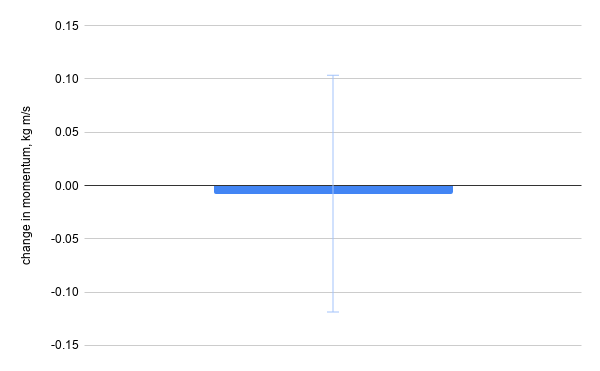
\includegraphics[width=4in]{dmomentum.png}
\end{center}
\caption{Example bar plot of change in momentum; $\Delta p = \SI{-0.007\pm0.06}{\kilo\gram\meter\per\second}$. Yours may look different.}
\label{fig:momentum-change}
\end{figure}

\end{document}